\documentclass[12pt,preprint]{aastex61}
\textwidth  6.5in
\textheight 9in
\oddsidemargin -0.1cm          
\evensidemargin -0.1cm
\topmargin -1.2cm
\usepackage{times}
\usepackage{graphicx}
\input epsf
\parskip = 2pt

\begin{document}

\begin{center}
\vspace{0.2in}\underline{\Large AST 381: Planetary Astrophysics}\\
\large Final Exam, Due Sunday Dec 17 before midnight\\
\end{center}

\vspace{-0.1in} This is a take-home exam, due by Sunday Dec 17 via email. It is open notes/reading/internet/everything, but no talking to other people or comparing materials. Answers should be formulated in your own words, no block quotes, etc etc. Note that in general, the specific answer is easy. It's the justification that you need to put some time into.

There are 6 questions here. You should answer 3 of them. Each answer should be a page or so - use more if you need it, but I'm trying to calibrate the level of effort you should put into this. For ease and consistency, feel free to just type your answers into this latex document and compile it, then turn in the latex and PDF, plus any supporting figures. If you'd like clarification on something, just ask.

{\bf 1. On a plot of $\log(M_{planet})$ versus $\log(a_{planet})$, sketch out the ranges of parameter space where planets can be found using RV (current technology), transit (Kepler), and astrometry (Gaia). Use order-of-magnitude arguments or calculations to justify the overall shape and locations of the detection limit for each curve.}

For simplicity, assuming the star is sun-like, i.e. 1 solar mass and 1 solar radius. Also, given that we have only been looking for planets for about 20 years, and we need to observe a planet for a full cycle to validate the discovery, any planets with more than 8 AU ($\approx 10^{12}$ m) are not considered.

For the RV method, we'll assume that the minimum radial velocity magnitude the current technology can detect is approximately 10 m/s. The radial velocity of the star, assuming the planet is in an edge-on, circular orbit, is as followed:

\begin{equation}
v_* = \frac{2\pi a_*}{P} = \frac{2\pi}{2\pi\sqrt{\frac{a^3}{GM_*}}}\frac{M_p}{M_*}a = \sqrt{\frac{G}{M_*a}} M_p \approx 6\times10^{-21} \frac{M_p}{\sqrt{a}} \geq 10
\end{equation}
where $M_p$ is in kg, and $a$ is in m, and further algebra yields that $M_p \geq 2\times10^{22} \sqrt{a}$.

For the transit method, we'll say 20 ppm is the detection limit, and as before, assuming the planet is in an edge-on, circular orbit. The reduction in luminosity can be calculated as:

\begin{equation}
\rho = \left( \frac{R_p}{R_*} \right)^2 \geq 2\times10^{-5}
\end{equation}
and further algebra will yield $ R_p \geq 4\times 10^{-2} R_* \approx 3000$ km. Assuming rocky planet, the minimum mass would then be $ 3\times 10^{23}$ kg. Note that the semi-major axis is not relevant for this method.

For the astrometry method, the Gaia spacecraft is expected to be able to detect down to 20 mas, and assuming the average stars are approximately 100 pc. Assume the planet is in a face-on circular orbit. The angular distance traveled by the star can be calculated as:

\begin{equation}
\theta = \frac{1}{d}\frac{M_p}{M_*}a \geq \frac{2\times 10^{-5}}{3600}
\end{equation}
and further algebra yields $M_pa \geq \frac{0.02}{3600} M_* d \approx 3 \times 10^{44}  $.

Combining these results into a plot, and we get:

\begin{figure}[h]
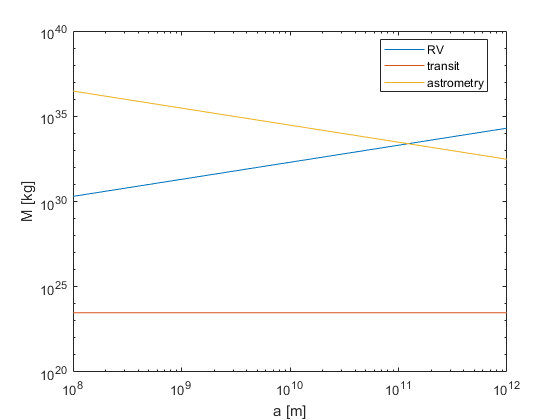
\includegraphics[scale=1]{prob1_plot.png}
\caption{$M_{planet}$ vs $a_{planet}$}
\centering	
\end{figure}

{\bf 2. Describe the observational process of producing a ``transit spectrum''. What sets the amplitude of the measurement, in terms of the atmospheric properties of the transiting planet (temperature, surface gravity, atmospheric composition, etc), and what would this characteristic scale be for the Earth?}

(skipped)

{\bf 3. Why do we think that dust in debris disks must be constantly replenished, and using scaling arguments, justify why we think mass is initially locked in large objects but then flows efficiently down to the smallest sizes. What ultimately removes dust grains from the system?}

(skipped)

{\bf 4. What is the Jeans mass, and how does its functional dependence on density naturally lead to the production of star clusters? What is the observational downfall of trying to claim that all stars form near the Jeans mass in molecular clouds? What change in local conditions sets the smallest scale on which fragmentation occurs, below which no further subdivision occurs?}

(skipped)

{\bf 5. Describe the process by which a bunch of 1 km sized rock+ice boulders in a disk ultimately turn into a Jupiter, noting the major points where behavior changes. You can assume this is happening just outside the ice line. You don't need to rigorously derive a timescale, or the size-scales where interesting things happen, but describe hand-wavily how you would derive those quantities.}

At first, the only way for two boulders to combine is for collisions between them to occur, and this could either lead to fragmentation or aggregation of the two boulders, depending on the relatively velocity and the structure of the two boulders. If aggregation occurs, the gravitational force would be able to mold it into spherical shape. As more mass is added to the proto-planet, the gravitational force due to the planet would allow it to not only absorb boulders that are on direct collision course, but also absorb the ones that will fall into the gravitational well of the proto-planet, known as gravitation focusing. 

At some point, the planet grows so much that the gravitational focusing phenomenon causes the planet to grow exponentially. This is called the runaway growth, and this occurs when the cross-sectional area within which the planet can attract object is larger than twice of planet's cross-sectional area. 

After more growth, the planet eventually reach about 20 $M_\Earth$, at which point the planet can start holding on gases like hydrogen and helium. When this occur, the planet becomes a gas giant, and the growth will not stop until it has gathered all the material in its orbital vicinity.

{\bf 6. What are some of the current ideas on how planets can migrate from their formation sites? What are some observational signatures that might indicate which mode accounts for the majority of cases?}

{\bf Type I migration} 

In this case, the planet produces an anomaly in the gravitational field such that the dusts fall into a pair of spiral arms around the planet. The spiral arms will generate a force on the planet and slow it down, thus shrinking the orbit. Since this migration occurs while the dust is still present, the material will still be accreting onto the planet. However, while this seems to be an essential transition state between having protoplanetary disk and planets, with the current understanding of this mechanism, it should be highly unlikely that a planet can form in this fashion and survive the early stage: the inward migration rate is too high for the migration to stop before the planet falls into the star. 

With the current understanding of Type I migration, we should see only a small number of stars with planets.

{\bf Type II migration}
Once the planet has gathered enough material to have its Hill's radius be larger than the thickness of the protoplanetary disk at its orbit, the planet will clear a gap in the disk. When this occurs, the force acting on the planet will reduce dramatically, thus leading to the planet moving inward at a much slower rate. In this case, the migration will stop when the planet reaches the magnetosphere of the star. 

An observational signature for this is the abundance of hot Jupiters, as they have to form further away from the star, and slowly move towards the star. Another evidence would be seeing most of the planets being more or less co-planar with the star's equator, as this mechanism does not involve the planet leaving the equatorial plane.
 
 
{\bf Kozai mechanism}

A distant object (i.e. gas giant, companion star) provides a perturbation torque that makes the orbit of the planet precesses (trading between inclination and eccentricity).

An evidence for this would be the misalignment between the star's rotation and the planet's orbit.
\end{document}

